\documentclass[10pt]{article}

\pagestyle{plain}
\textwidth 6.5 in
\oddsidemargin 0 in
\evensidemargin 0 in
\topmargin 0 in
\textheight 8 in

\pagestyle{empty}

\usepackage[all]{xy}
\usepackage{graphicx}
\usepackage{units}
\usepackage{enumerate}
\usepackage[hidelinks]{hyperref}

\usepackage{amssymb, amsmath, pict2e}
 \pagestyle{myheadings}

\usepackage{pdfsync}
\usepackage{rotating}
\usepackage{multirow}
\usepackage[normalem]{ulem}
\usepackage{cancel}

\usepackage{color}
\usepackage[usenames,dvipsnames,svgnames,table]{xcolor}
\usepackage{pgf,tikz}
\usetikzlibrary{arrows}
\usepackage{environ}
\usepackage{environ}
\makeatletter
\newsavebox{\measure@tikzpicture}
\NewEnviron{scaletikzpicturetowidth}[1]{%
  \def\tikz@width{#1}%
  \def\tikzscale{1}\begin{lrbox}{\measure@tikzpicture}%
  \BODY
  \end{lrbox}%
  \pgfmathparse{#1/\wd\measure@tikzpicture}%
  \edef\tikzscale{\pgfmathresult}%
  \BODY
}


\title{Characterization and complexity of Thin Strip Graphs}

\author{Abdeselam El-Haman Abdeselam \\  Department of Computer Science \\ Universite Libre de Bruxelles}


\date{May 7, 2014}

%%%%%%%%%%%%%%%%  start macros  %%%%%%%%%%%%%%%%%%%%%%%%%%%%%%%%%
\newtheorem{theorem}{Theorem}
\newtheorem{defn}[theorem]{Definition}
\newtheorem{example}[theorem]{Example}
\newtheorem{remark}[theorem]{Remark}
\newtheorem{question}[theorem]{Question}

\newtheorem{lemma}[theorem]{Lemma}
\newtheorem{claim}[theorem]{Claim}
\newtheorem{prop}[theorem]{Proposition}
\newtheorem{corollary}[theorem]{Corollary}
\newtheorem{conjecture}[theorem]{Conjecture}

\newtheorem{hyp}[theorem]{Hypothesis}
\newtheorem{alg}[theorem]{Algorithm}

\newcommand{\qed}{\mbox{$\Box$}}
\newcommand{\proof}{\medbreak\par\noindent{\bf Proof. }}
 \newcommand{\GP}{{\vec{G}}_P}
\newcommand{\GN}{{\vec{G}}_N}

\newcommand{\cover}{\mathrel{\rlap{$\prec$}
                                \rlap{\hskip 0.7em $\cdot$}
                                 \phantom{\prec}}}

\newcommand{\re}{re}

\newcommand{\up}{\mbox{\rm{up}}}
\newcommand{\side}{\mbox{\rm{side}}}
\newcommand{\type}{\mbox{\rm{type}}}


\def\reals{{\mathbb R}}


\newcommand{\ahat}{{\hat{a}}}
\newcommand{\bhat}{{\hat{b}}}
\newcommand{\chat}{{\hat{c}}}
\newcommand{\dhat}{{\hat{d}}}
\newcommand{\bolda}{{\bf{a}}}
\newcommand{\boldb}{{\bf{b}}}
\newcommand{\boldc}{{\bf{c}}}
\newcommand{\boldd}{{\bf{d}}}

\newcommand{\iplus}{{\cal I}^+}
\newcommand{\iminus}{{\cal I}^-}
\newcommand{\ipm}{{\cal I}^{\pm}}
\newcommand{\ipmix}{{\cal I}^{{\cal M}}}

\newcommand{\upl}{{\cal U}^+}
\newcommand{\uminus}{{\cal U}^-}
\newcommand{\upm}{{\cal U}^{\pm}}
\newcommand{\upmix}{{\cal U}^{{\cal M}}}


\newcommand{\ppl}{{\cal P}^+}
\newcommand{\pminus}{{\cal P}^-}
\newcommand{\ppm}{{\cal P}^{\pm}}
\newcommand{\ppmix}{{\cal P}^{{\cal M}}}
\newcommand{\bpm}{{\cal B}^{\pm}}
\newcommand{\tpm}{{\cal T}^{\pm}}
\newcommand{\bpmix}{{\cal B}^{{\cal M}}}
\newcommand{\tpmix}{{\cal T}^{{\cal M}}}
%%%%%%%%%%%%%%%%  end macros  %%%%%%%%%%%%%%%%%%%%%%%%%%%%%%%%%

\begin{document}

  \maketitle

\bibliographystyle{plain}


\begin{center} {\sl ABSTRACT} \end{center}

\begin{quotation}

Abstract

\end{quotation}

%% This is an example first chapter.  You should put chapter/appendix that you
%% write into a separate file, and add a line \include{yourfilename} to
%% main.tex, where `yourfilename.tex' is the name of the chapter/appendix file.
%% You can process specific files by typing their names in at the
%% \files=
%% prompt when you run the file main.tex through LaTeX.
\section{Graphs and disks}
\label{sec:graphs}


\subsection{Graphs}

A graph $G$ is defined as $G = (V,E)$, where $V$ is the set of vertices and $E$ the set of
edges, where $E \subseteq \binom{V}{2}$. The vertices $v,w \in V$ such that $e = vw \in E$
links are called the \textit{endpoints} of $e$.

\begin{defn}
  An embedding of a graph $G$ into a surface $\Sigma$ is a mapping of $G$ in
  $\Sigma$ where the vertices correspond to distinct points and the edges
  correspond to simple arcs connecting the images of their endpoints.
  \cite{goyalGraphEmbeddingTechniques2017}.
\end{defn}

A graph $G$ is planar if there is an embedding of this graph that does not have
any crossing between the edges.

\begin{defn}
  Let $G = (V,E)$ and $S \subset V$, an induced subgraph is a graph $H$ of $G$ whose
  vertex set is $S$ and its edge set $F = \{vw : v,w \in S, vw \in E\}$.
\end{defn}

\begin{defn}
  $H$ is called a \textit{minor} of $G$ if $H$ can be constructed by deleting edges and vertices,
  or contracting edges.
\end{defn}

In graph theory, (forbidden graph characterization)...

\begin{theorem}[Kuratowski]
  A graph $G$ is planar if and only if it doesn't contain $K_5$ or $K_{3,3}$ as a minor or
  a induced subgraph.
\end{theorem}


\subsection{Intersection graphs}

\begin{defn}
The \textit{intersection graph} of a collection $\zeta$ of objects is the graph
$(\zeta,E)$ such that $c_1c_2\in E \Leftrightarrow c_1 \cap c_2 \neq \varnothing$.
\end{defn}


\begin{defn}
  A partial order set is a binary relation $\leq$ over a set $A$ satisfying these axioms:
  \begin{itemize}
    \item $a \leq a$ (reflexivity).
    \item if $a \leq b$ and $b \leq a$ then $a = b$ (antisymmetry).
    \item if $a \leq b$ and $b \leq c$ then $a \leq c$ (transitivity).
  \end{itemize}
\end{defn}

\begin{defn}
   A partially ordered set or poset  $(S,\leq)$ where $S$ a set and $\leq$ a partial
   order on $S$.
\end{defn}

\begin{defn}
  A graph $G$ is a comparibility graph if for each edge $\{u,v\} \in E$ there is
  a binary relation $R$ such that $u \leq v$ or $v \leq u$. Equivalently, $G$
  is a comparability graph if it is the comparability graph of a poset. For
  example, the Hasse diagram (figure \ref{fig:hasse}) is a comparability graph
  where the relation is inclusion.
\end{defn}

\begin{figure}
\centering

\begin{scaletikzpicturetowidth}{\textwidth}
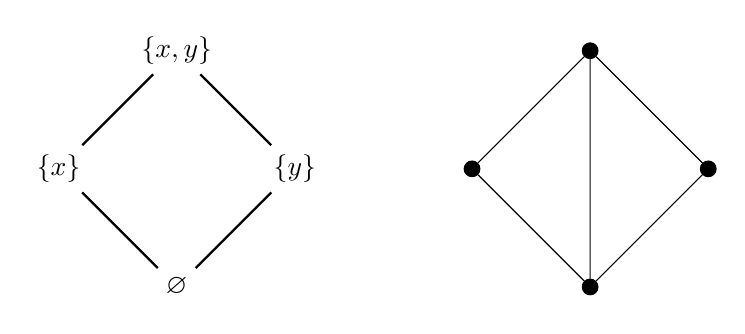
\begin{tikzpicture}[scale=1.5]

  % poset
  \draw (-1cm,0cm) node (v2) {$\{x\}$};
  \draw (1cm,0cm)  node (v3) { $\{y\}$ };
  \draw (0cm,-1cm) node (v4) {$\varnothing$};
  \draw (0cm,1cm)  node (v1) {$\{x,y\}$};

  \draw[thick]  (v1) edge (v2);
  \draw[thick]  (v3) edge (v1);
  \draw[thick]  (v3) edge (v4);
  \draw[thick]  (v2) edge (v4);

  % graph
  \node[draw,circle,inner sep=2pt,fill,label distance=1cm] (v1g) at (3.5,1) {};
  \node[draw,circle,inner sep=2pt,fill,label distance=1cm] (v2g) at (3.5,-1) {};
  \node[draw,circle,inner sep=2pt,fill,label distance=1cm] (v3g) at (4.5,0) {};
  \node[draw,circle,inner sep=2pt,fill,label distance=1cm] (v4g) at (2.5,0) {};
  \draw  (v1g) edge (v2g);
  \draw  (v1g) edge (v4g);
  \draw  (v4g) edge (v2g);
  \draw  (v1g) edge (v3g);
  \draw  (v3g) edge (v2g);

\end{tikzpicture}
\end{scaletikzpicturetowidth}

\caption{On the left, Hasse diagram of a poset of the power set of 2 elements ordered by inclusion.
On the right, the comparability graph of this poset.}
\label{fig:hasse}
\end{figure}

\subsubsection{Interval graphs}

Definition of interval Graphs

Properties

Definition of MIXED interval graphs


\subsection{Realizations}

\begin{defn}
  A graph $G$ is said \textit{realizable} if
\end{defn}

The \textit{graph realizability problem} is the problem that finds a realization
of a given length $l(e)$ for a graph $G$ (this means that the edge $e$ has to
be represented by a straight line of length $l(e)$ in $\mathbb{R}^2$).

A unit distance graph $G$ is a graph that has a realization where 2 points $u,v$
have $\text{dist}(u,v) = 1$ if and only if their respective vertices are adjacent.
This problem  will be shown at chapter \ref{sec:complex} to be $\exists
\mathbb{R}$-complete. If  this realization doesn't have any crossing then $G$ is a
\textit{matchstick graph}.\\

A unit disk graph $G$ is a graph that has a realization where 2 points have
$\text{dist}(u,v) \leq 1$ if and only if their respective vertices are adjacent.
Each point can be represented as the center of a disk of unit diameter and the
edges can be represented as the intersection of 2 disks. This class of graphs
is important for this thesis, as the Thin Strip Graphs are a sub-class of
Unit Disk Graphs (section \ref{sec:thin}). Unit Disk Graph realizability is
$\exists \mathbb{R}$-complete. We will refer to the Unit Disk Graph class as
UDG and an example of a realization can be found in the figure \ref{fig:udg}.

% Figure about the K_1,3 construction
\begin{figure}
\centering

\begin{scaletikzpicturetowidth}{\textwidth}
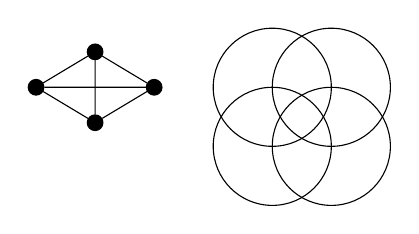
\begin{tikzpicture}[scale=1.5]

  \draw (-0.5,2.5) circle [radius=0.5];
  \draw (0,2.5) circle [radius=0.5];
  \draw (-0.5,2) circle [radius=0.5];
  \draw (0,2) circle [radius=0.5];


  \node[draw,circle,inner sep=2pt,fill,label distance=1cm] (v1) at (-2.5,2.5) {};

  \node[draw,circle,inner sep=2pt,fill,label distance=1cm] (v2) at (-2,2.2) {};
  \node[draw,circle,inner sep=2pt,fill,label distance=1cm] (v3) at (-2,2.8) {};
  \node[draw,circle,inner sep=2pt,fill,label distance=1cm] (v4) at (-1.5,2.5) {};

  \draw  (v3) edge (v2);
  \draw  (v4) edge (v1);
  \draw  (v3) edge (v1);
  \draw  (v4) edge (v2);
  \draw  (v3) edge (v4);
  \draw  (v1) edge (v2);

\end{tikzpicture}
\end{scaletikzpicturetowidth}

\caption{Realization of a UDG (Unit Disk Graph).}
\label{fig:udg}
\end{figure}

%% This is an example first chapter.  You should put chapter/appendix that you
%% write into a separate file, and add a line \include{yourfilename} to
%% main.tex, where `yourfilename.tex' is the name of the chapter/appendix file.
%% You can process specific files by typing their names in at the
%% \files=
%% prompt when you run the file main.tex through LaTeX.
\section{Complexity}
\label{sec:complex}

Complexity theory has the objective to establish lower bounds on how efficient
an algorithm can be for a given problem \cite{sipser2006}. This approach let us
have a reference point to establish the difficulty of a problem.


\begin{defn}
Let $\Sigma$ be a finite alphabet, $\Sigma^*$ every word derived from $\Sigma$, $L \subseteq \Sigma^*$ is a decision problem.
\end{defn}

\begin{defn}
The algorithm $A$ decides problem $L \subseteq \Sigma^*$ if for all word $w \in \Sigma^*$:
\begin{itemize}
  \item $A$ finishes and returns TRUE if $w \in L$.
  \item $A$ finishes and returns FALSE if $w \notin L$.
\end{itemize}
\end{defn}

\begin{defn}
A problem is verifiable if there's an algorithm that verifies it.
\end{defn}

\begin{defn}
A problem is decidable if there's an algorithm that decides it.
\end{defn}

\subsection{P vs NP}

\begin{defn}
A problem $L \in \mathcal{P}$ if $L$ can be decided in polynomial time $\mathcal{O}(n^k)$.
\end{defn}

\begin{defn}
A problem $L \in \mathcal{NP}$ if $L$ can be verified in polynomial time
$\mathcal{O}(n^k)$. Thus, $\mathcal{P} \subseteq \mathcal{NP}$.
\end{defn}

To prove a bound of complexity on an unknown problem $L$ we have to find other
problems with already known complexity and find equivalences between those 2. This
can be achieved through \textit{reductions}.

\begin{defn}
  A reduction of a problem $L$ to a problem $M$ is a mapping of an instance of $L$ ($I_L$)
  to an isntance of $M$ ($I_M$) such that $I_L$ is true for the problem $L$ if and
  only if $I_M$ is true for the problem $M$. This is noted $L \leq M$ and $L \leq_P M$
  if the reduction is done in polynomial time.
\end{defn}

With this concept we can define new complexity classes. $\mathcal{NP}$-hard is
the set of problems so that we can reduce every $\mathcal{NP}$ problem to. The set
of problems that are $\mathcal{NP}$-hard and $\mathcal{NP}$ are called $\mathcal{NP}$-complete.
This is generalized to every complexity class ($\mathcal{P}$, $\exists \mathbb{R}$, RP, etc...)

\paragraph{Satisfiability problem} The satisfiability problem (SAT) decides the satisfiability
of a CNF formula $\phi$. A CNF formula is a boolean formula that is a conjunction of multiple
clauses $c_k$. A clause is a disjunction of multiple litterals. A litteral may be a variable
or a negation of a variable.

\begin{theorem}[Cook-Levin]
  SAT is $\mathcal{NP}$-complete.
\end{theorem}

\subsection{$\exists \mathbb{R}$ complexity class}

$\exists \mathbb{R}$ is the class that describes the problems that can be reduced to \textit{the existential theory of the reals}\cite{ExistentialTheoryReals2006}. The decidability of the existential theory of the reals is the problem that decides if a sentence of this form is true:

$$(\exists X_1 \dots \exists X_n): F(\exists X_1, \dots,\exists X_n)$$\\

where $F$ is a quantifier-free formula in the reals. In other words, it's a
conjuntion of clauses where each clause is a real polynomial inequality where
each variable $X_k$ is a real number. We can see that ETR is NP-hard because
SAT can be reduced to it.


\begin{proof}
  Let's take an instance of SAT $\phi_{SAT}$ with clauses $c_k$ and variables
  $x_k$, we can construct an instance of ETR $\phi_{ETR}$ where we can
  construct variables in the domain $\{0,1\}$ with this equality, so for each
  variable $X_k$:
  $$X_k - X_k^2 = 0$$

  Each litteral of each clause will be positive or negative depending if the litteral is cancelled in $\phi_{SAT}$:

  $$x_k \to l = X_k$$
  $$\neg x_k \to l = -X_k$$

  Then for each clause we can have a polynomial that will sum the value of every litteral in the clause must be greater that one, so that at least one litteral is true:

  $$\sum_{l\in c_k} l \geq 1$$

  With this proof, it's easy to see that $\phi_{ETR}$ is valid if and only if $\phi_{SAT}$ is also valid.  \qed\\

\end{proof}

This result can show us that $P \subseteq NP \subseteq \exists \mathbb{R}$.

\subsubsection{Problems in $\exists \mathbb{R}$}

In this section we will describe some problems that are $\exists
\mathbb{R}$-complete and will give an overview about the proof since it is
not the main goal of this paper (donner détail de pourquoi je donne un
overview).

\paragraph{The art gallery problem} Given a simple polygon $P$ (without
crossings between every side), we introduce \textit{guards}. A guard $g$ is
a point that every point of the polygon is watched by a guard. A point
$p$ is watched by a point $q$ if the segment $pq$ is contained in $P$. The
subset $G$, being $G$ the set of guards and $G \subseteq P$, is optimum if it
has the minimal cardinality covering the whole polygon.

The art gallery problem decides given a polygon $P$ and a number of guards $k$
if there exists a configuration of $k$ guards in $G$ guarding the whole
polygon. The art gallery problem is $\exists \mathbb{R}$-complete
\cite{abrahamsenArtGalleryProblem2017}.

\paragraph{Proof idea} First of all, we can see that the art gallery problem
is in $\exists \mathbb{R}$ if we reduce this problem to ETR. If we have an
instance $(P,k)$ of the art gallery problem we can have a formula
\cite{EFRAT2006238} like this:

$$\phi = \{\exists x_1y_1,\dots x_ky_k \forall p_xp_y :
\text{INSIDE-POLYGON}(p_x,p_y) \to \bigvee_{1 \leq i \leq k}
\text{SEES}(x_i,y_i,p_x,p_y)\}$$

Where INSIDE-POLYGON returns $1$ if $(p_x,p_y) \in P$ and SEES returns $1$ if
the segment $(x,y)(p_x,p_y) \in P$. $\phi$ is not a ETR formula, so we'd like
to construct a quantifier-free formula with the idea of $\phi$. To achieve this,
the main idea is to have a small set of points $Q \subseteq P$ such that if these
points are watched, the whole polygon is watched. This subset $Q$ is called
the \textit{witness set}. The only thing is now to create a polynome for each
point that ensures the point is watched by a guard.

To finish the proof we have to prove that the art gallery problem is $\exists
\mathbb{R}$-hard. For this part an $\exists \mathbb{R}$-complete
problem has been deducted from ETR. For the problem ETR-INV we have a set of
variables $\{x_1,\dots,x_n\}$ and a set of equations of this form:

$$x = 1,\ \ x + y = z,\ \ x \cdot y = 1 $$

and the problem decides if it exists a solution to this set of equations such
that the value of each variable is real in $[\frac{1}{2},2]$.

A reduction of ETR-INV is found to the art gallery problem by constructing
a polygon $P$ and finding a number $g$ for that polygon such that the instance
of ETR-INT is true if and only if $P$ is covered by at most $g$ guards.

\paragraph{Unit Disk Graph recognition} The Unit Disk Graph recognition is
the problem that decides if a graph $G$ has a realization $\phi$ as a Unit
Disk Graph. Unit Disk Graph recognition is $\exists \mathbb{R}$-complete.

Recognition of Unit Disk Graphs is $\exists \mathbb{R}$-complete. (corollary of graph realizability problem)\cite{Schaefer2013}

Stretchability is $\exists \mathbb{R}$-complete.

%% This is an example first chapter.  You should put chapter/appendix that you
%% write into a separate file, and add a line \include{yourfilename} to
%% main.tex, where `yourfilename.tex' is the name of the chapter/appendix file.
%% You can process specific files by typing their names in at the
%% \files=
%% prompt when you run the file main.tex through LaTeX.
\section{Geometry}
\label{sec:geom}


\section{Thin Strip Graphs}

\subsection{Stabbing disks}

Definition of stabbing.

Stabbing geometric structures.\cite{schlipf2013stabbing}

\subsection{Thin Strip Graphs}

$c$-strip graphs are unit disk graphs such that the centers of the disks are delimited on the area $\{(x,y) : -\infty < x < \infty, 0 < y \leq c\}$ and its class noted SG($c$). We can say that SG(0) = UIG and SG($\infty$) = UDG. \cite{hayashiThinStripGraphs2017}

\begin{defn}
  Thin strip graphs are defined as TSG $= \bigcap_{c > 0}$ SG($c$).
\end{defn}

\begin{remark}
  SG($0$) $\neq$ TSG. We can construct a $K_{1,3}$ such that we have 3 vertices with the coordinates
  $(1,0)$, $(0,0)$, $(1,0)$ and a last one $(0,\varepsilon)$ with $\varepsilon > 0$ as seen in Figure \ref{fig:thinK13}.
\end{remark}


% Figure about the K_1,3 construction
\begin{figure}
\centering

\begin{scaletikzpicturetowidth}{\textwidth}
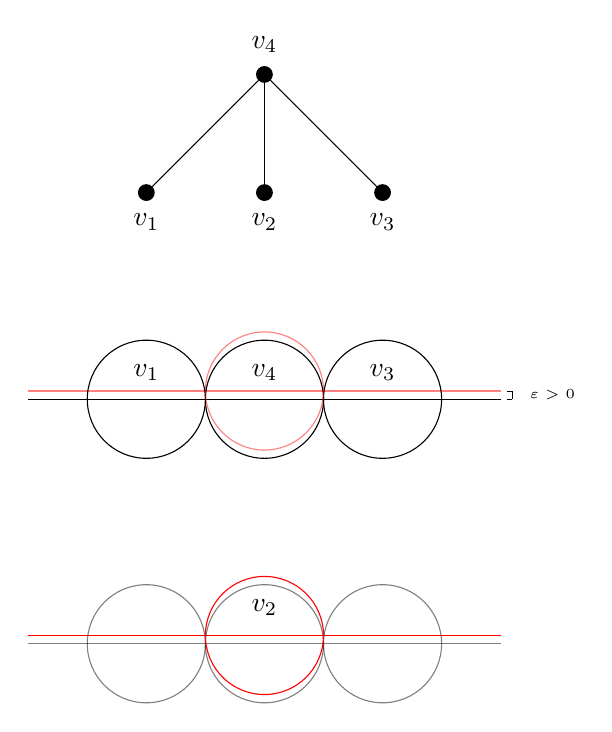
\begin{tikzpicture}[scale=1.5]

\draw (-2,0) -- (2,0);
\draw[red ,opacity = 0.5] (-2,0.07) -- (2,0.07);
\draw  (-1,0) circle [radius=0.5];
\draw[color=black] (-1,0.2265) node {$v_1$};
\draw  (0,0) circle [radius=0.5];
\draw[color=black] (0,0.2265) node {$v_4$};
\draw  (1,0) circle [radius=0.5];
\draw[color=black] (1,0.2265) node {$v_3$};

\draw[red, opacity = 0.5] (0,0.07) circle [radius=0.5];

\draw[color=black] (2.4386,0.0367) node {\tiny $\varepsilon > 0$};

% lines to describe distance (epsilon)
\draw[very thin] (2.1,0.07) -- (2.1,0);
\draw[very thin] (2.05,0.07) -- (2.1,0.07);
\draw[very thin] (2.05,0) -- (2.1,0);

\draw[opacity = 0.5] (-2,-2.07) -- (2,-2.07);
\draw[red] (-2,-2) -- (2,-2);
\draw[opacity = 0.5]  (0,-2.07) circle [radius=0.5];
\draw[opacity = 0.5]  (1,-2.07) circle [radius=0.5];
\draw[opacity = 0.5]  (-1,-2.07) circle [radius=0.5];
\draw[red] (0,-2) circle [radius=0.5];
\draw[color=black] (0,-1.765) node {$v_2$};

\node[draw,circle,inner sep=2pt,fill,label distance=1cm] (v1) at (0,2.75) {};
\draw[color=black] (0,3) node {$v_4$};
\node[draw,circle,inner sep=2pt,fill,label distance=1cm] (v3) at (0,1.75) {};
\draw[color=black] (0,1.5) node {$v_2$};
\node[draw,circle,inner sep=2pt,fill,label distance=1cm] (v2) at (-1,1.75) {};
\draw[color=black] (1,1.5) node {$v_3$};
\node[draw,circle,inner sep=2pt,fill,label distance=1cm] (v4) at (1,1.75) {};
\draw[color=black] (-1,1.5) node {$v_1$};
\draw  (v1) edge (v2);
\draw  (v1) edge (v3);
\draw  (v1) edge (v4);
\end{tikzpicture}
\end{scaletikzpicturetowidth}

\caption{A construction of $K_{1,3}$ with a disk realization, being this graph a TSG.}
\label{fig:thinK13}
\end{figure}

It has been proven that MUIG $\subsetneq$ TSG.\\


Denote that there's not constant $t$ such that SG($t$) = TSG.\\

Unfettered unit interval graphs = UUIG\\

MUIG $\subsetneq$ TSG $\subsetneq$ UUIG\\

UUIG $\subseteq$ co-comparability graphs (to prove).

In the following sections we state the problems that are being studied for the thesis.

\subsubsection{Forbidden subgraphs of Thin Strip Graphs}
  We've proven that MUIG $\subsetneq$ TSG $\subsetneq$ UUIG. Knowing the\\
  (Why $F_k$ is a co-comparability unit disk graph?)

\subsubsection{Complexity class of TSG recognition}
  We've shown in section \ref{sec:complex} that some intersection geometric
  problems are in $\exists \mathbb{R}$ (unit disk graph recognition problem or
  the art gallery problem) and we'd like to know if
  TSG recognition or even SG($c$) recognition is in $NP$ knowing that TSG
  $\subseteq$ UDG.


\bibliography{main}

\end{document}
